\documentclass[a4paper,12pt]{article}

\usepackage{amssymb}
\usepackage{amsmath}
\usepackage{amsfonts}
\usepackage{txfonts}
\usepackage{upgreek}
\usepackage{graphicx}
\usepackage{siunitx}
\usepackage{enumerate}
\usepackage[left=2cm,right=2cm,top=2cm,bottom=2cm]{geometry}

\usepackage[obeyspaces]{url}

%\newcommand{\question}[2]{\textbf{\textit{#1}}\quad{\footnotesize\textit{(#2 points)}}\\[3mm]}
\newcommand{\question}[1]{\textbf{\textit{#1}}}
\newcommand{\points}[1]{\quad{\footnotesize\textit{(#1 points)}}}
\newcommand{\point}{\quad{\footnotesize\textit{(1 point)}}}
\newcommand{\HRule}{\rule{\linewidth}{0.3mm}}
\newcommand{\dd}{\mathrm{d}}
\renewcommand{\pi}{\uppi}
\newcommand{\ii}{\mathrm{i}}
\renewcommand{\thefootnote}{\normalsize\fnsymbol{footnote}}
\DeclareMathOperator{\e}{e}
\newcommand{\bra}{\langle}
\newcommand{\ket}{\rangle}

\renewcommand{\theequation}{\Roman{equation}}

\begin{document}
\pagestyle{empty}

\begin{center}
\LARGE \textbf{Astronomy from 4 perspectives: the Dark Universe}
\HRule
\end{center}
\begin{flushright}
prepared by: Jena participants and BMS
\end{flushright}
\begin{center}
{\Large \textbf{play with data: rotation curves of galaxies}}
\end{center}
\vspace{5mm}

\noindent
Observations of the rotation of disc galaxies is nowadays done in the H$\alpha$-line of hydrogen, because it reaches to much larger distances from the galaxy centre compare to the stellar light. In this exercise we have a look at a data set on low surface-brightness galaxies by W. de Blok, S. McGaugh and V. Rubin, Astronomical Journal 122, 2381 (2001).

\begin{enumerate}[\itshape \bfseries 1.]

\item \question{flat rotation curves}\\
Let's start by exploring H$\alpha$-data for low surface-brightness galaxies.
\begin{enumerate}[(a)]
\item{Why is it a clever idea to focus on galaxies with a low (optical) surface brightness?}
\item{What is the general relationship between rotation curve $\upsilon(r)$ and mass profile $\rho(r)$?}
\item{A isothermal sphere with a core has the density profile $\rho(r)$,
\begin{equation}
\rho(r) = \rho_0\left(1+\left(\frac{r}{r_c}\right)^2\right)^{-1},
\end{equation}
with the central density $\rho$ and the core radius $r_c$. The corresponding velocity profile $\upsilon(r)$,
\begin{equation}
\upsilon(r)^2 = 4\pi G\rho_0 r_c^2\left(1-\frac{r_c}{r}\arctan\left(\frac{r}{r_c}\right)\right),
\end{equation}
with the gravitational constant $G\simeq 10^{-11}~\mathrm{m}^3/\mathrm{kg}/\mathrm{s}^2$.}
\item{Please show that the asymptotic value for $\upsilon$ for $r\rightarrow\infty$ is $\upsilon_\infty = \sqrt{4\pi G\rho_0r_c^2}$. Please check the units of the relation between $\upsilon_\infty$ and $r_c$ and $\rho_0$.}
\item{Please use the script \path{rotplot.py} and plot a couple of rotation curves: Do they show the expected behaviour?}
\end{enumerate}

\begin{figure}[h]
\begin{center}
\resizebox{9cm}{!}{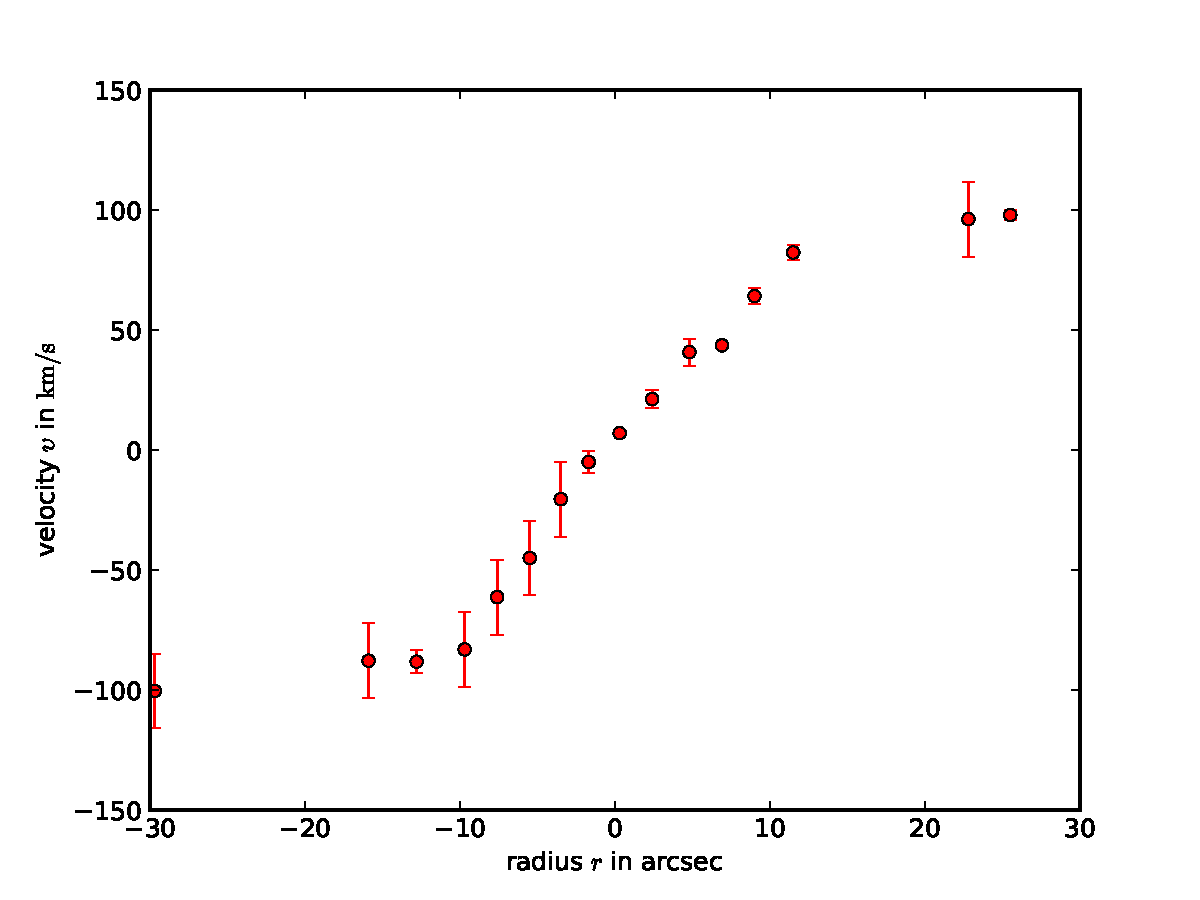
\includegraphics{./figures/rotplot.pdf}}
\caption{rotation curve $\upsilon(r)$ of the galaxy F568}
\end{center}
\end{figure}

\item \question{luminous and dark matter}\\
With the script \path{rotfit.py} you can fit a model rotation curve to data. Take care to read off the distance $d$ to the galaxy from the table, in order to convert $r$ from arcseconds to $\mathrm{kpc}$.
\begin{enumerate}[(a)]
\item{Are the curves from the isothermal-sphere model providing a good fit to data?}
\item{What are typical velocities $\upsilon_\infty$, central densities $\rho_0$ and core radii $r_c$?}
\item{What is the role of $\epsilon$ in the script? Why are the results not affected if $\epsilon$ is small enough?}
\end{enumerate}
Please continue by completing the table.
\begin{enumerate}[(a)]
\setcounter{enumii}{3}
\item{Please try to find out if the mass to light-ratio $M/L$ is large: For that purpose, estimate the total mass $M$ in units of the solar mass $M_\odot = 10^{30}~\mathrm{kg}$,
\begin{equation}
M = 4\pi\int_0^\infty r^2\mathrm{d}r\: \rho(r),
\end{equation}
and compare it to the total luminosity. For the integral, you can use the result
\begin{equation}
\int\dd x\:\frac{x^2}{1+x^2} = \arctan(x) + \mathrm{const}.
\end{equation}
Please truncate the integration at the tidal radius $10r_c$. With the expression for the mass, please verify the relationship between orbital velocity $\upsilon$ and distance $r$.
}
\item{Then, please express the mass to light-ratio $M/L$ in units of solar masses per solar luminosities $M_\odot/L_\odot$: The luminosity $L$ in units of the solar luminosity $L_\odot$ follows from the difference of the absolute magnitudes,
\begin{equation}
\frac{L}{L_\odot} = 10^{0.4(\mathrm{Mag}_\odot - \mathrm{Mag})},
\end{equation}
you can find the values for $\mathrm{Mag}$ of the galaxies in the table, and use the literature value for $\mathrm{Mag}_\odot=5.45$ in the same band ($R$-band) from the literature.
}
\item{Is there evidence for dark matter?}
\end{enumerate}

\begin{figure}[h]
\begin{center}
\resizebox{9cm}{!}{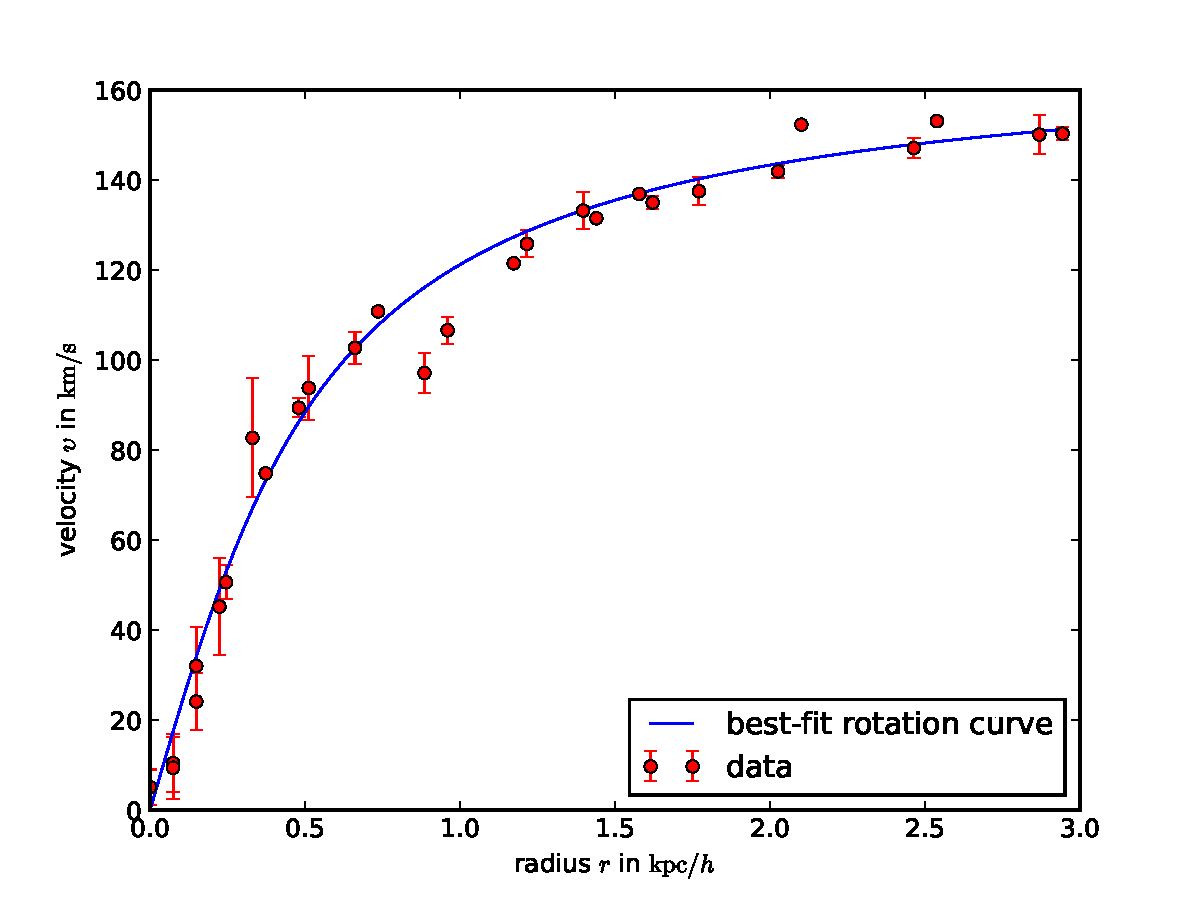
\includegraphics{./figures/rotfit.pdf}}
\caption{fit of a isothermal sphere rotation curve $\upsilon(r)$ to the galaxy U11557 at 22 Mpc distance, with the values $r_c=0.412~\mathrm{kpc}$ and $\upsilon_\infty = 169~\mathrm{km}/\mathrm{s}$.}
\end{center}
\end{figure}

\begin{table}[h]
\begin{center}
\begin{tabular}{|l|r|r|r|r|r|r|r|}
\hline
galaxy		& $d$ in $\mathrm{Mpc}$	& $\upsilon_\infty$ in $\mathrm{km}/\mathrm{s}$ & $r_c$ in $\mathrm{kpc}$ & $M$ in $M_\odot$ & $\mathrm{Mag}$ & $M/L$ in $M_\odot/L_\odot$\\
\hline
E0140040	& 212	& & & & -21.6 & \\
E0840411	& 80	& & & & -18.1 & \\
E1200211	& 15	& & & & -15.6 & \\
E1870510	& 18	& & & & -16.5 & \\
E2060140	& 60	& & & & -19.2 & \\
E3020120	& 69	& & & & -19.1 & \\
E3050090	& 11	& & & & -17.3 & \\
E4250180	& 86	& & & & -20.5 & \\
E4880049	& 22	& & & & -16.8 & \\
F563-1		& 45	& & & & -17.3 & \\
F568-3		& 77	& & & & -18.3 & \\
F571-8		& 48	& & & & -17.6 & \\
F579-V1		& 85	& & & & -18.8 & \\
F583-1		& 32	& & & & -16.5 & \\
F583-4		& 49	& & & & -16.9 & \\
U4115		& 3.2	& & & & -12.4 & \\
U5750		& 56	& & & & -18.7 & \\
U6614		& 85	& & & & -20.3 & \\
U11454		& 91	& & & & -18.6 & \\
U11557		& 22	& 169 & 0.412 & & -20.0 & \\
U11583		& 5		& & & & -14.0 & \\
U11616		& 73	& & & & -20.3 & \\
U11648		& 48	& & & & -21.0 & \\
U11748		& 73	& & & & -22.9 & \\
U11819		& 60	& & & & -20.3 & \\
\hline
\end{tabular}
\end{center}
\end{table}


\end{enumerate}
\end{document}
